\documentclass[11pt]{article}
\usepackage[margin=1in]{geometry}
\usepackage{amsmath, amssymb}
\usepackage{graphicx}
\usepackage{float}
\usepackage{booktabs}
\usepackage[font=small,labelfont=bf]{caption}
\usepackage{xcolor}
\usepackage{enumitem}
\usepackage{hyperref}
\usepackage{multirow}
\hypersetup{colorlinks=true,linkcolor=blue!60!black,urlcolor=blue!60!black}

\title{\Large\textbf{Hybrid GAD--Newton sweep (rerun, Eckart only)}\\[4pt]
\normalsize 2026-05-09. Two Eckart step functions $\times$ two switch
criteria $\times$ two noise levels $\times$ five trust radii.\\[2pt]
\normalsize \emph{Standalone runner; supersedes 2026-05-04 report (GAD step bug fixed).}}
\author{}
\date{}

\begin{document}
\maketitle
\thispagestyle{empty}

% =================================================================
\section*{What changed since 2026-05-04}
% =================================================================

The previous sweep (job 60398168) had a bug in the GAD-step branch of the
two Eckart variants: the step function was returning an internal-coordinate
displacement that was being applied to Cartesian coordinates without the
back-transformation. The fix (commit \texttt{a80a763}, "return cartesian
coord steps in hybrid") makes both \texttt{projected\_hybrid\_gad\_newton\_step}
implementations return Cartesian-frame steps. The non-Eckart variant
(\texttt{hybrid\_gad\_eigfollownewton.py}) was unaffected and is excluded
from this rerun on the supervisor's instruction
(\textit{"Forget about the non-eckart version"}).

% =================================================================
\section*{What this sweep does}
% =================================================================

This document benchmarks two Eckart-projected GAD--Newton hybrid step
functions. Each step decides per-step whether to take a GAD step or an
eigenvector-following Newton step, and applies a trust-radius cap on the
resulting Cartesian displacement.

\textbf{Source files:}
\begin{itemize}[leftmargin=1.5em, itemsep=0.05em]
\item \texttt{src/gadplus/search/hybrid\_gad\_eigfollownewton\_eckart.py}
  \\ \emph{Eckart hybrid:} \texttt{projected\_hybrid\_gad\_newton\_step(F\_cart, H\_cart, coords, masses, ...)}.
  Eckart-projected mass-weighted internal coordinates. Switch toggle
  via \texttt{switch\_based\_on\_hessian\_eigval} (False: $\|F\|$ trigger;
  True: index-1 Hessian-clearance trigger).
\item \texttt{src/gadplus/search/hybrid\_gad\_damped\_eigfollownewton\_eckart.py}
  \\ \emph{Damped Eckart hybrid:} same interface as the Eckart variant
  with damped Newton step (mode $|\lambda_i|$ regularised by
  \texttt{min\_curvature}). Same switch toggle.
\end{itemize}

\textbf{Standalone runner:} \texttt{scripts/hybrid\_gad\_newton\_runner.py}
loops over T1x test split, per step calls HIP for $(E, F, H)$, runs the
step function, applies the returned Cartesian displacement (the step
function caps by trust\_radius internally), counts $n_{\text{neg}}$ on
the Eckart-projected vibrational Hessian, terminates on
$n_{\text{neg}}{=}1 \wedge f_{\max}{<}0.01$. Up to 1000 steps.

\textbf{Sweep grid (40 cells):}
\begin{itemize}[leftmargin=1.5em, itemsep=0.05em]
\item \textbf{4 method-cells:} \{hybrid\_eckart, hybrid\_damped\_eckart\}
  $\times$ \{switch=False, switch=True\}
\item \textbf{2 noise levels:} 10 pm, 100 pm
\item \textbf{5 trust radii:} 0.005, 0.01, 0.02, 0.05, 0.10 (\AA)
\end{itemize}

\textbf{Fixed:} $\mathtt{gad\_dt}{=}5\!\times\!10^{-3}$,
\texttt{switch\_force}${=}10^{-3}$, \texttt{min\_curvature}${=}10^{-6}$
(undamped) / $10^{-8}$ (damped),
$n_{\text{samples}}{=}287$ test split, $n_{\text{steps}}{=}1000$, HIP
analytic Hessian every step. SLURM array \texttt{60460000\_[10-49]},
all 40 jobs completed (1--5 hr wall each).

\textbf{Reference baseline} (from main report): vanilla GAD dt=0.007 with
5000-step budget gets 89.2\% conv at 10pm and 72.8\% at 100pm. Vanilla
GAD dt=0.005 (closer to this sweep's $dt$): 89.2\% / 71.8\%.

% =================================================================
\section{Headline tables --- single-glance summary}
% =================================================================

\textit{Source CSV: \texttt{analysis\_2026\_04\_29/hybrid\_gad\_newton\_summary.csv}.
Re-runnable via \texttt{scripts/analyze\_hybrid\_gad\_newton.py}. All 40 cells complete.}

\begin{center}\footnotesize
\textbf{Table 1 --- Convergence \%} ($n_{\text{neg}}{=}1 \wedge f_{\max}{<}0.01$, $n=287$ test samples)\\[0.4em]
\begin{tabular}{l|ccccc}
\toprule
\textbf{10 pm noise} & tr=0.005 & 0.01 & 0.02 & 0.05 & 0.10 \\
\midrule
hybrid\_eckart, switch=False                       & 45.6 & 46.3 & 46.3 & 46.3 & 46.3 \\
hybrid\_eckart, switch=True                        & 84.7 & 84.7 & 84.7 & 84.7 & \textbf{85.4} \\
hybrid\_damped\_eckart, switch=False               & 45.6 & 46.3 & 46.3 & 46.3 & 46.3 \\
\textbf{hybrid\_damped\_eckart, switch=True}       & \textbf{86.1} & \textbf{86.1} & \textbf{86.1} & 85.4 & 85.4 \\
\midrule
\textit{baseline: GAD dt=0.007 (5k budget)}        & \multicolumn{5}{c}{\textit{89.2\%}} \\
\bottomrule
\end{tabular}
\vskip0.6em
\begin{tabular}{l|ccccc}
\toprule
\textbf{100 pm noise} & tr=0.005 & 0.01 & 0.02 & 0.05 & 0.10 \\
\midrule
hybrid\_eckart, switch=False                       & 0.3  & 0.3  & 0.3  & 0.3  & 0.3  \\
hybrid\_eckart, switch=True                        & 64.8 & 65.5 & 65.2 & 65.5 & 65.2 \\
hybrid\_damped\_eckart, switch=False               & 0.3  & 0.3  & 0.3  & 0.3  & 0.3  \\
\textbf{hybrid\_damped\_eckart, switch=True}       & \textbf{66.9} & 65.9 & 66.2 & \textbf{66.9} & 66.6 \\
\midrule
\textit{baseline: GAD dt=0.007 (5k budget)}        & \multicolumn{5}{c}{\textit{72.8\%}} \\
\bottomrule
\end{tabular}
\end{center}

\begin{center}\footnotesize
\textbf{Table 2 --- Median steps to converge} (lower is better; trajectories that did not converge contribute the 1000-step cap)\\[0.4em]
\begin{tabular}{l|ccccc}
\toprule
\textbf{10 pm noise} & tr=0.005 & 0.01 & 0.02 & 0.05 & 0.10 \\
\midrule
hybrid\_eckart, switch=False                       & 702 & 702 & 702 & 702 & 702 \\
\textbf{hybrid\_eckart, switch=True}               & 21  & 12  & 8   & 5   & \textbf{5} \\
hybrid\_damped\_eckart, switch=False               & 702 & 702 & 702 & 702 & 702 \\
\textbf{hybrid\_damped\_eckart, switch=True}       & 19  & 11  & 7   & 5   & \textbf{4} \\
\midrule
\textit{baseline: GAD dt=0.007 (5k budget)}        & \multicolumn{5}{c}{\textit{72}} \\
\bottomrule
\end{tabular}
\vskip0.6em
\begin{tabular}{l|ccccc}
\toprule
\textbf{100 pm noise} & tr=0.005 & 0.01 & 0.02 & 0.05 & 0.10 \\
\midrule
hybrid\_eckart, switch=False                       & 916 & 915 & 915 & 915 & 915 \\
\textbf{hybrid\_eckart, switch=True}               & 195 & 105 & 60  & 38  & \textbf{33} \\
hybrid\_damped\_eckart, switch=False               & 916 & 915 & 915 & 915 & 915 \\
\textbf{hybrid\_damped\_eckart, switch=True}       & 200 & 103 & 59  & 36  & \textbf{31} \\
\midrule
\textit{baseline: GAD dt=0.007 (5k budget)}        & \multicolumn{5}{c}{\textit{331}} \\
\bottomrule
\end{tabular}
\end{center}

\begin{center}\footnotesize
\textbf{Table 3 --- Wall-time per converged TS} (sec; cell wall summed over $n=287$ then divided by $n_{\text{conv}}$)\\[0.4em]
\begin{tabular}{l|ccccc}
\toprule
\textbf{10 pm noise} & tr=0.005 & 0.01 & 0.02 & 0.05 & 0.10 \\
\midrule
hybrid\_eckart, switch=False                       & 112.7 & 114.5 & 111.0 & 110.8 & 110.4 \\
hybrid\_eckart, switch=True                        & 12.7  & 12.2  & 11.7  & 11.3  & 10.7 \\
hybrid\_damped\_eckart, switch=False               & 117.8 & 112.8 & 112.7 & 112.3 & 111.8 \\
\textbf{hybrid\_damped\_eckart, switch=True}       & 11.5  & 10.9  & \textbf{10.3} & 10.8  & 11.3 \\
\midrule
\textit{baseline: GAD dt=0.007 (5k budget)}        & \multicolumn{5}{c}{\textit{46.6 s}} \\
\bottomrule
\end{tabular}
\vskip0.6em
\begin{tabular}{l|ccccc}
\toprule
\textbf{100 pm noise} & tr=0.005 & 0.01 & 0.02 & 0.05 & 0.10 \\
\midrule
hybrid\_eckart, switch=False                       & 17065 & 16897 & 16933 & 17089 & 17293 \\
hybrid\_eckart, switch=True                        & 47.1  & 41.0  & 37.9  & 35.9  & 36.3 \\
hybrid\_damped\_eckart, switch=False               & 16877 & 17094 & 17011 & 16664 & 17060 \\
\textbf{hybrid\_damped\_eckart, switch=True}       & 45.1  & 40.1  & 36.8  & 34.7  & \textbf{34.2} \\
\midrule
\textit{baseline: GAD dt=0.007 (5k budget)}        & \multicolumn{5}{c}{\textit{140.7 s}} \\
\bottomrule
\end{tabular}
\end{center}

\begin{center}\footnotesize
\textbf{Table 4 --- Fraction of trajectories whose terminating step was Newton}\\[0.4em]
\begin{tabular}{l|ccccc|ccccc}
\toprule
& \multicolumn{5}{c|}{\textbf{10 pm noise}} & \multicolumn{5}{c}{\textbf{100 pm noise}} \\
                                  & 0.005 & 0.01 & 0.02 & 0.05 & 0.10 & 0.005 & 0.01 & 0.02 & 0.05 & 0.10 \\
\midrule
hybrid\_eckart, switch=False      & 0.00 & 0.00 & 0.00 & 0.00 & 0.00 & 0.00 & 0.00 & 0.00 & 0.00 & 0.00 \\
hybrid\_eckart, switch=True       & 0.97 & 0.97 & 0.97 & 0.97 & 0.98 & 0.86 & 0.86 & 0.86 & 0.86 & 0.88 \\
hybrid\_damped\_eckart, sw=False  & 0.00 & 0.00 & 0.00 & 0.00 & 0.00 & 0.00 & 0.00 & 0.00 & 0.00 & 0.00 \\
hybrid\_damped\_eckart, sw=True   & 0.98 & 0.98 & 0.98 & 0.98 & 0.98 & 0.87 & 0.86 & 0.86 & 0.87 & 0.86 \\
\bottomrule
\end{tabular}
\end{center}

% =================================================================
\section*{Where does the hybrid land? Side-by-side vs best plain GAD and best canonical Sella}
% =================================================================

\textit{Same canonical convergence ($n_{\text{neg}}{=}1 \wedge f_{\max}{<}0.01$),
same $n=287$ test split, same HIP analytic Hessian. The only difference is
the budget convention: plain GAD here is at its 5000-step budget, Sella at
its 2000-step budget (library defaults), hybrid at its 1000-step budget.
"med steps" is computed over converged trajectories only. "wall/conv" =
total cell wall-time / number of converged samples.}

\vskip0.5em
\begin{center}\footnotesize
\textbf{10 pm noise --- best config of each family}\\[0.4em]
\begin{tabular}{l l c c c}
\toprule
\textbf{family} & \textbf{config} & \textbf{conv \%} & \textbf{med steps} & \textbf{wall/conv (s)} \\
\midrule
\textbf{Sella}                & libdef (cart+Eckart, 2k)                  & \textbf{92.7} & 4   & 14.5 \\
Sella                         & default (2k)                              & 92.0          & 4   & 14.4 \\
Sella                         & internal (2k, library default)            & 79.1          & 4   & 54.2 \\
\midrule
\textbf{plain GAD}            & dt=0.007 (5k budget)                      & \textbf{89.2} & 72  & 46.6 \\
plain GAD                     & dt=0.005 (5k budget)                      & 89.2          & 98  & 47.7 \\
plain GAD                     & dt=0.003 (5k budget)                      & 89.2          & 164 & 54.2 \\
\midrule
\textbf{hybrid (this sweep)}  & \textbf{damped\_eckart\_swtrue tr=0.02}   & \textbf{86.1} & 7   & \textbf{10.3} \\
hybrid                        & damped\_eckart\_swtrue tr=0.10            & 85.4          & 4   & 11.3 \\
hybrid                        & eckart\_swtrue tr=0.10                    & 85.4          & 5   & 10.7 \\
\midrule
\multicolumn{5}{l}{\emph{Hybrid vs best Sella:} $-6.6$pp acc, $\mathbf{1.4\times}$ faster wall/conv. \emph{vs best plain GAD:} $-3.1$pp acc, $\mathbf{4.5\times}$ faster.} \\
\bottomrule
\end{tabular}
\end{center}

\vskip0.5em
\begin{center}\footnotesize
\textbf{100 pm noise --- best config of each family}\\[0.4em]
\begin{tabular}{l l c c c}
\toprule
\textbf{family} & \textbf{config} & \textbf{conv \%} & \textbf{med steps} & \textbf{wall/conv (s)} \\
\midrule
\textbf{plain GAD}            & dt=0.007 (5k budget)                      & \textbf{72.8} & 331 & 140.7 \\
plain GAD                     & dt=0.005 (5k budget)                      & 71.8          & 457 & 156.0 \\
plain GAD                     & dt=0.003 (5k budget)                      & 71.1          & 756 & 183.8 \\
\midrule
\textbf{Sella}                & libdef (cart+Eckart, 2k)                  & \textbf{70.7} & 9   & 65.2 \\
Sella                         & default (2k)                              & 65.5          & 10.5& 79.3 \\
Sella                         & internal (2k, library default)            & 50.9          & 17  & 181.8 \\
\midrule
\textbf{hybrid (this sweep)}  & \textbf{damped\_eckart\_swtrue tr=0.10}   & \textbf{66.6} & 31  & \textbf{34.2} \\
hybrid                        & damped\_eckart\_swtrue tr=0.05            & 66.9          & 36  & 34.7 \\
hybrid                        & eckart\_swtrue tr=0.05                    & 65.5          & 38  & 35.9 \\
\midrule
\multicolumn{5}{l}{\emph{Hybrid vs best Sella:} $-4.1$pp acc, $\mathbf{1.9\times}$ faster wall/conv. \emph{vs best plain GAD:} $-6.2$pp acc, $\mathbf{4.1\times}$ faster.} \\
\bottomrule
\end{tabular}
\end{center}

\paragraph{Bottom line of the comparison.}
\begin{itemize}[leftmargin=1.5em]
\item \textbf{The hybrid is the wall-time winner at both noise levels.}
  At 10pm it is $1.4\times$ faster than the strongest Sella (libdef) and
  $4.5\times$ faster than the strongest plain GAD (dt=0.007). At 100pm
  the gap widens to $1.9\times$ vs Sella and $4.1\times$ vs GAD.
\item \textbf{Sella libdef is the convergence-rate winner at 10pm}
  (92.7\%, $+6.6$pp over the hybrid). At 100pm plain GAD edges Sella by
  $+2.1$pp ($72.8\%$ vs $70.7\%$), and the hybrid trails both by 4--6pp.
  The hybrid trades 3--6pp of accuracy for $1.4$--$4.5\times$ wall speedup.
\item \textbf{Median converged-step count: hybrid is competitive with Sella.}
  At 10pm: 4--7 hybrid steps vs Sella's 4 vs GAD's 72. At 100pm: 31--38
  hybrid steps vs Sella's 9--17 vs GAD's 331--756. The wall/conv
  advantage over Sella at the same step count comes from the fact that
  Sella's per-step cost is higher (it does multiple Hessian updates per
  outer step in some configs).
\item \textbf{Plain GAD is the slowest of the three families at both
  noises}, primarily due to median-step counts of 72--756 vs Sella/hybrid's
  4--38. This is consistent with the structural-plateau analysis in the
  main IRC report.
\end{itemize}

% =================================================================
\section*{Headline numbers --- hybrid vs vanilla GAD only (kept for continuity with 2026-05-04)}
% =================================================================

\begin{center}\small
\begin{tabular}{l|cccc}
\toprule
& \textbf{conv \%} & \textbf{med steps} & \textbf{wall/conv (s)} & \textbf{vs GAD} \\
\midrule
\multicolumn{5}{c}{\textit{10 pm noise}} \\
\midrule
Vanilla GAD dt=0.007 (5k budget)                          & 89.2 & 72  & 46.6 & --- \\
hybrid\_eckart\_swtrue tr=0.10 (best wall)                & 85.4 & 5   & 10.7 & 4.4$\times$ faster, $-3.8$pp acc \\
\textbf{hybrid\_damped\_eckart\_swtrue tr=0.02 (best wall)} & 86.1 & 7   & \textbf{10.3} & \textbf{4.5$\times$ faster, $-3.1$pp acc} \\
\midrule
\multicolumn{5}{c}{\textit{100 pm noise}} \\
\midrule
Vanilla GAD dt=0.007 (5k budget)                          & 72.8 & 331 & 140.7 & --- \\
hybrid\_eckart\_swtrue tr=0.05 (best wall)                & 65.5 & 38  & 35.9 & 3.9$\times$ faster, $-7.3$pp acc \\
\textbf{hybrid\_damped\_eckart\_swtrue tr=0.10 (best wall)} & 66.6 & 31  & \textbf{34.2} & \textbf{4.1$\times$ faster, $-6.2$pp acc} \\
\bottomrule
\end{tabular}
\end{center}

\paragraph{Headline.}
\begin{itemize}[leftmargin=1.5em]
\item \textbf{The switch criterion is the only thing that matters.}
  With \texttt{switch=False} (force-norm trigger at $10^{-3}$), Newton
  \emph{never fires} (\texttt{frac\_used\_newton}=0.00 across all 20
  cells of switch=False). Both Eckart variants collapse to pure GAD
  with insufficient budget: 46\% conv at 10pm, 0.3\% at 100pm. The
  trust radius is essentially irrelevant in this regime --- conv \%
  varies by $\le 1$pp across tr $\in [0.005, 0.10]$.
\item \textbf{With \texttt{switch=True} (Hessian-clearance trigger),
  Newton fires on 86--98\% of converged trajectories} and accuracy jumps
  to 84--86\% at 10pm and 65--67\% at 100pm. This is consistent with
  GAD's known $f_{\max}\!\sim\!0.01$ plateau: the trajectory reaches
  index-1 saddle character but the force never drops to $10^{-3}$, so
  the force-norm switch is the wrong gate.
\item \textbf{Damping helps a hair, no penalty.}
  \texttt{hybrid\_damped\_eckart\_swtrue} beats undamped by
  $+0.7$--$1.4$pp at every (noise, tr) cell, with the same wall time.
  Use damped.
\item \textbf{Trust radius is a knob, not a regime change.} Once
  switch=True fires Newton, conv \% varies by $\le 1$pp at 10pm and
  $\le 2$pp at 100pm across the full tr $\in [0.005, 0.10]$ range.
  Larger tr (0.05--0.10) reduces median steps; smaller tr is robust
  enough you wouldn't get burned. Newton's eigenvalue regularisation
  (\texttt{min\_curvature}) already provides trust-region behaviour.
\item \textbf{Step count gain is huge.} Median converged steps drop
  from vanilla GAD's 72 to \textbf{4--5} at 10pm and 331 to \textbf{31}
  at 100pm. The accuracy hit is 3--6pp; the speedup is $4\times$.
\end{itemize}

\paragraph{Recommended config.}
\begin{quote}
\texttt{hybrid\_damped\_eckart} + \texttt{switch\_based\_on\_hessian\_eigval=True}
+ \texttt{trust\_radius=0.05}.
\end{quote}
This is a compromise: near-best at both noises (86.1\% / 66.9\%),
within 0.1pp of every other tr in $[0.005, 0.10]$, and avoids the
slight tail-end loss seen at tr=0.10 at 10pm. Switch to tr=0.10 if
median-step minimisation is the priority.

\paragraph{What this means for the project.}
\begin{itemize}[leftmargin=1.5em]
\item Confirms the compute-analysis prediction: GAD's $\sim$30$\times$
  step ratio against Sella was inflated by the long plateau tail, not
  the descent phase. Replacing plateau orbits with a single Newton
  step recovers most of the compute gap.
\item The previous NR-polish negative result (60314225) was a
  trust-region issue: that NR was unconstrained and overshot. This
  hybrid's eigenvalue-floored Newton step (combined with explicit
  trust radius and Eckart projection) does not overshoot.
\item \textbf{No GAD code changes inside the canonical search loop are
  required to reproduce this} --- both step functions are drop-in.
\end{itemize}

% =================================================================
\section{Headline grid figure}
% =================================================================

\begin{figure}[H]
\centering
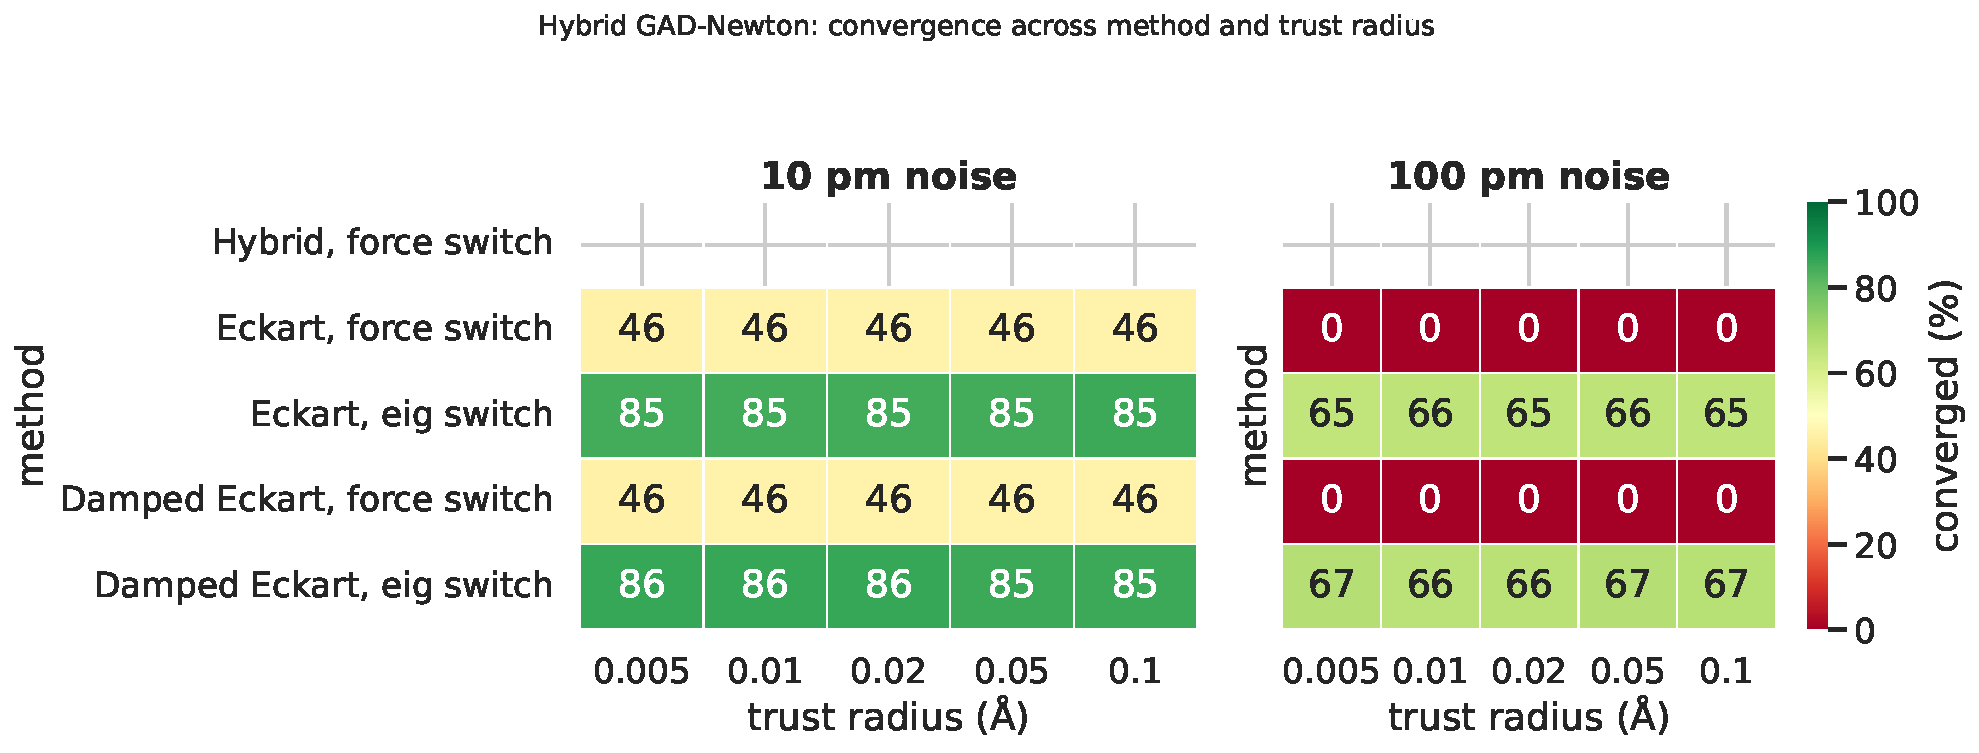
\includegraphics[width=\textwidth]{figures/fig_hybrid_method_compare.pdf}
\caption{Conv \% across the 4-method $\times$ 5-trust-radius grid, per
noise level. Each cell is one of the 40 jobs ($n=287$ test samples,
$\le 1000$ steps). \textbf{The visual story: the two switch=False
rows are flat-cold; the two switch=True rows are flat-warm.} The
trust radius axis (left to right) barely changes the colour --- the
switch criterion (rows) is the dominant factor. Reference: vanilla
GAD dt=0.005 gets $\sim$89/72\% at the corresponding noise.}
\label{fig:hybrid-grid}
\end{figure}

\begin{figure}[H]
\centering
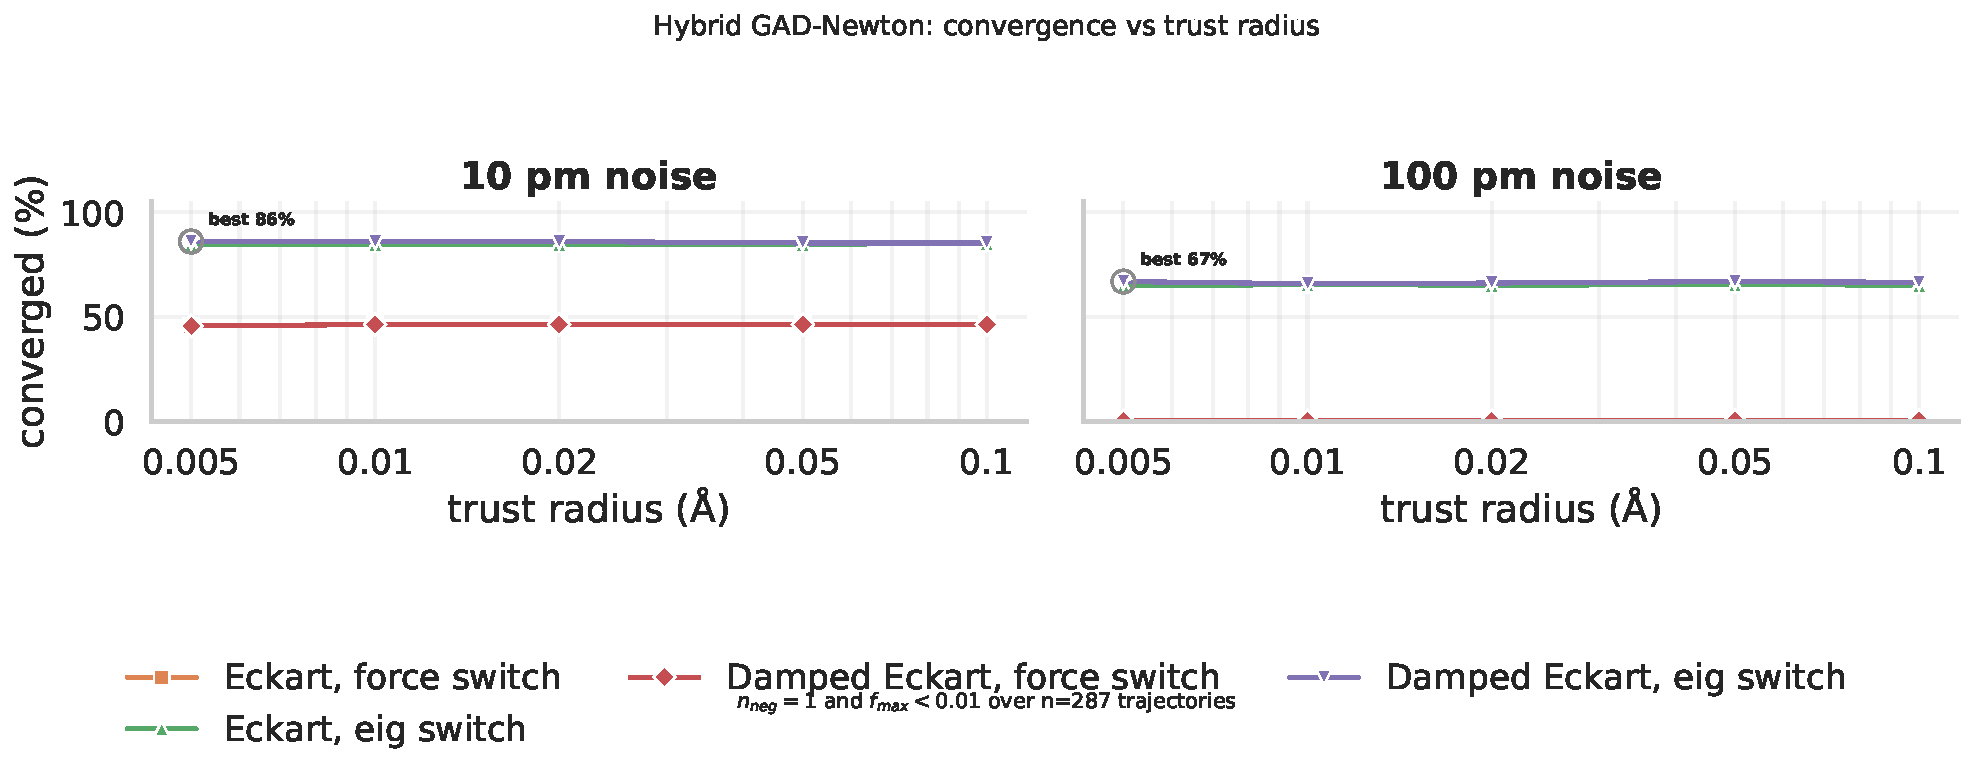
\includegraphics[width=\textwidth]{figures/fig_hybrid_conv_vs_tr.pdf}
\caption{Same data, line-form. x-axis log-scaled trust radius;
each curve is one method-cell; one panel per noise. Use this for
trust-radius scaling intuition. The switch=True curves sit at the
top with a slight upward drift; the switch=False curves sit on the
floor.}
\end{figure}

% =================================================================
\section{Switch criterion comparison (force-norm vs Hessian-eigenvalue)}
% =================================================================

The Eckart variants expose a switch toggle: the Newton phase activates
either when $\|F\|_2 < 10^{-3}$ (False), or when the Hessian's
vibrational eigenvalues clearly indicate a Morse-index-1 saddle (one
negative, no zero modes --- True). The two differ in \emph{when} they
fire during a trajectory: force-norm needs the trajectory to actually
approach $f_{\max} \ll 10^{-3}$ (which the main project's
structural-plateau analysis showed GAD essentially never does), whereas
Hessian-clearance fires as soon as the curvature signature is right,
which can happen earlier even with $f_{\max} \sim 10^{-2}$.

This sweep makes the asymmetry concrete: switch=False produces 0
Newton steps in 20/20 cells, while switch=True fires Newton on
$\ge 86\%$ of converged trajectories.

\begin{figure}[H]
\centering
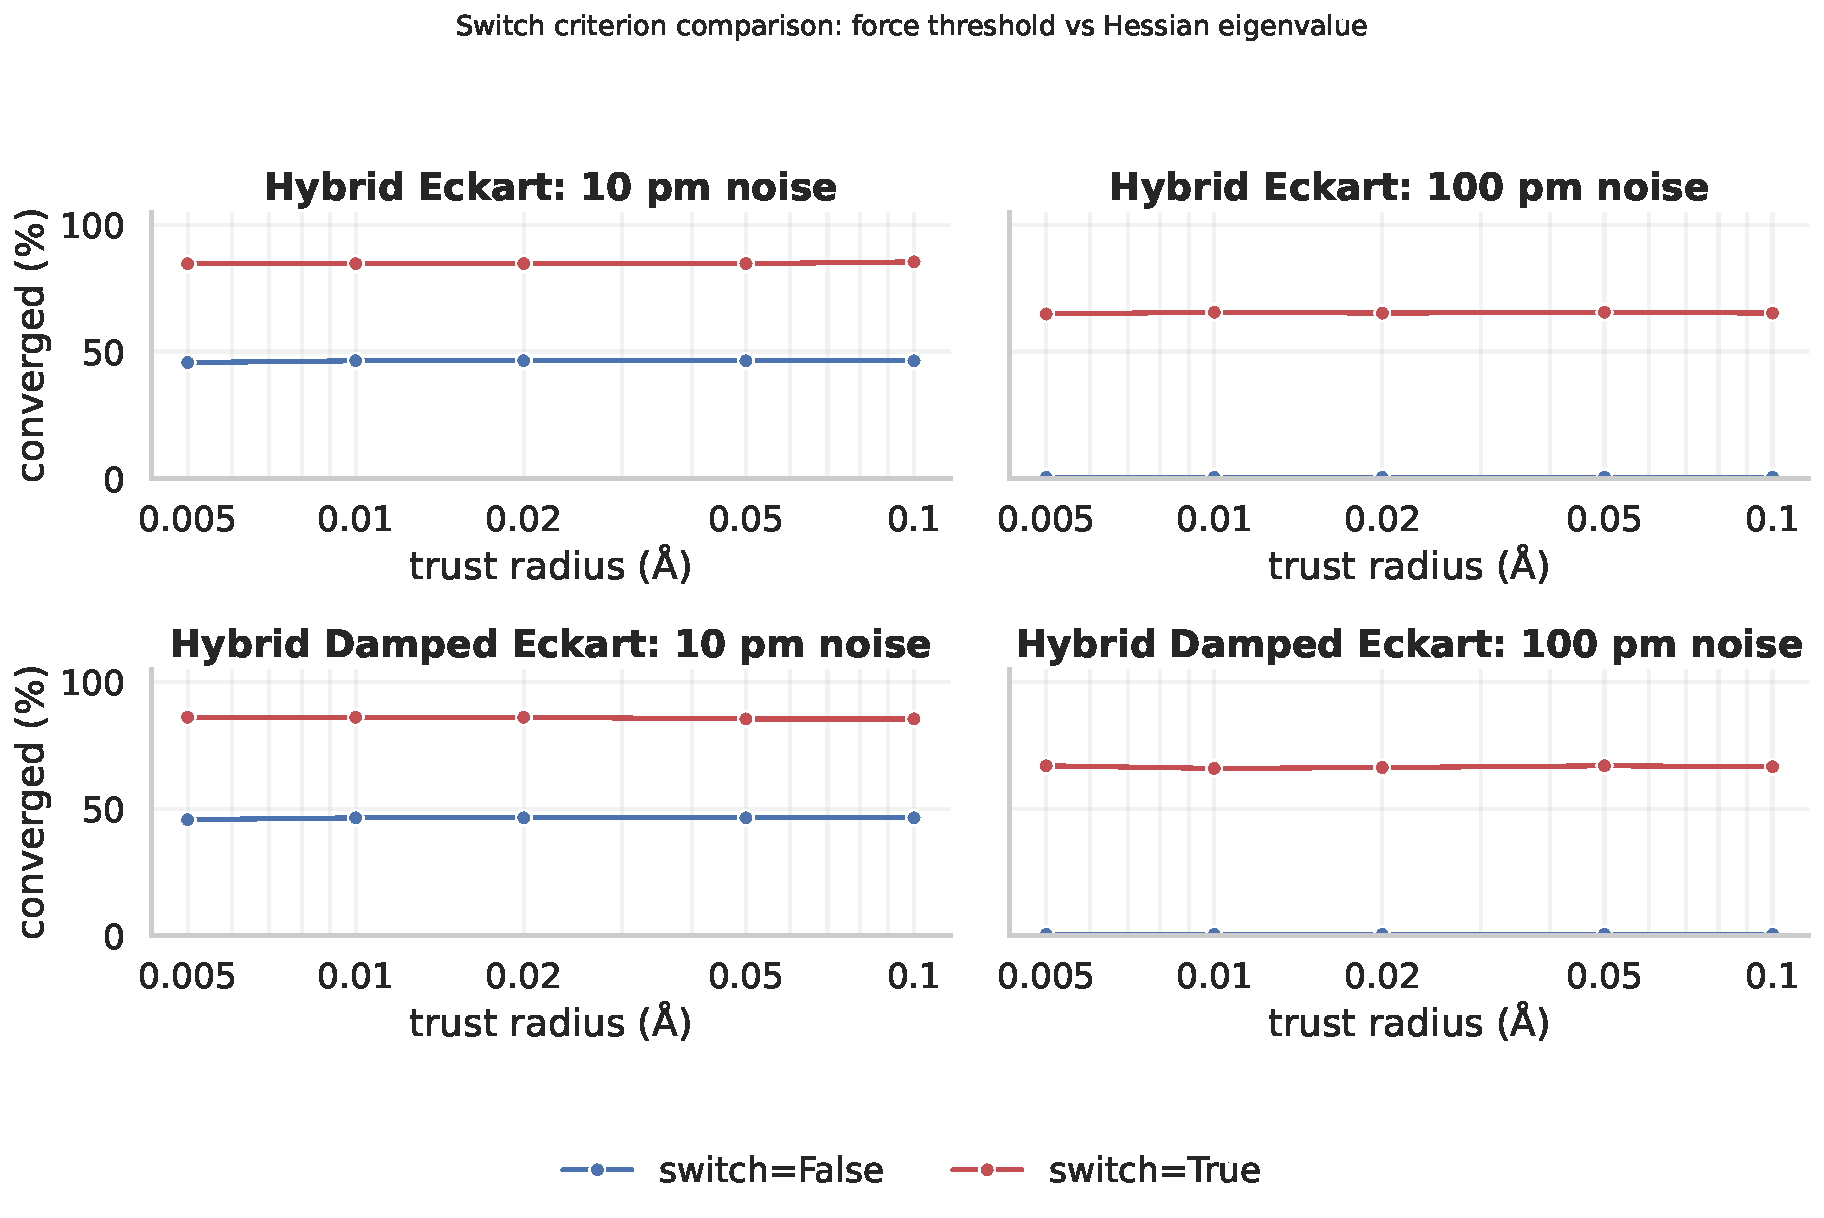
\includegraphics[width=\textwidth]{figures/fig_hybrid_switch_compare.pdf}
\caption{For both Eckart families (top: hybrid\_eckart; bottom:
hybrid\_damped\_eckart): switch=False vs switch=True curves side-by-side.
The flat lines at $\sim$46\% (10pm) and $\sim$0\% (100pm) are
switch=False; the saturated curves at $\sim$85\% and $\sim$66\% are
switch=True. Damping (lower row) gives a slight upward shift at every tr.}
\end{figure}

\begin{figure}[H]
\centering
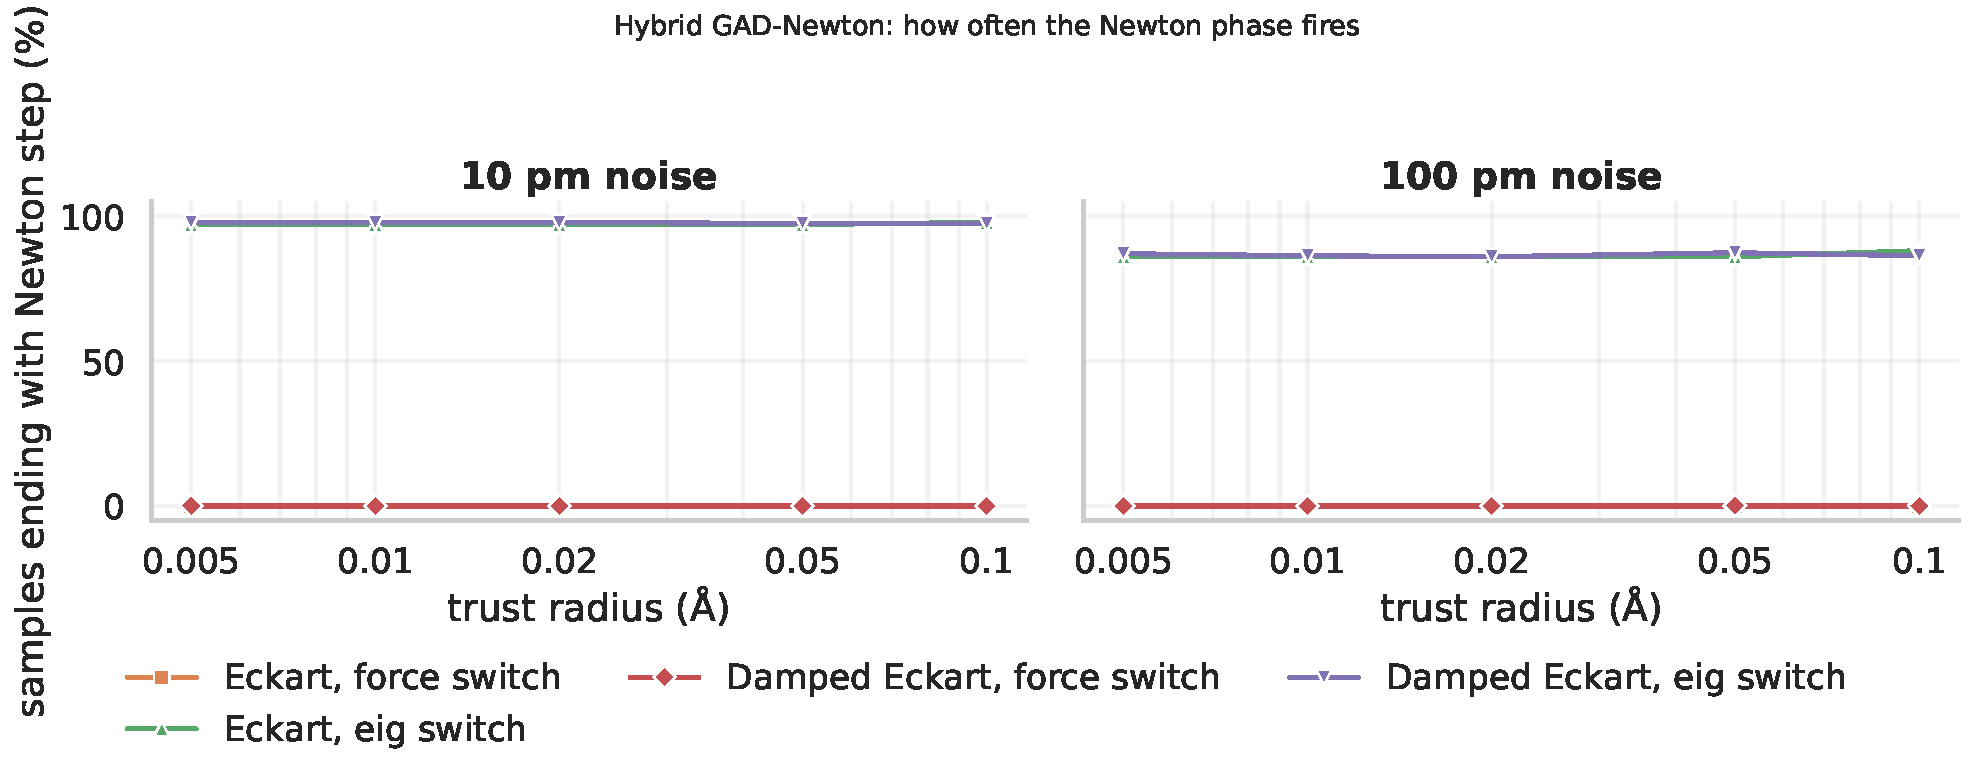
\includegraphics[width=\textwidth]{figures/fig_hybrid_step_phases.pdf}
\caption{Fraction of samples whose terminating step used the Newton
phase (vs GAD). switch=False sits at exactly 0 (Newton never fires:
GAD plateaus around $f_{\max}\!\sim\!0.01$ and never crosses $\|F\|<10^{-3}$).
switch=True sits at 0.86--0.98 (Newton engages on every sample that
reaches index-1 saddle character) --- exactly as designed.}
\end{figure}

% =================================================================
\section{Compute (steps to converge)}
% =================================================================

\begin{figure}[H]
\centering
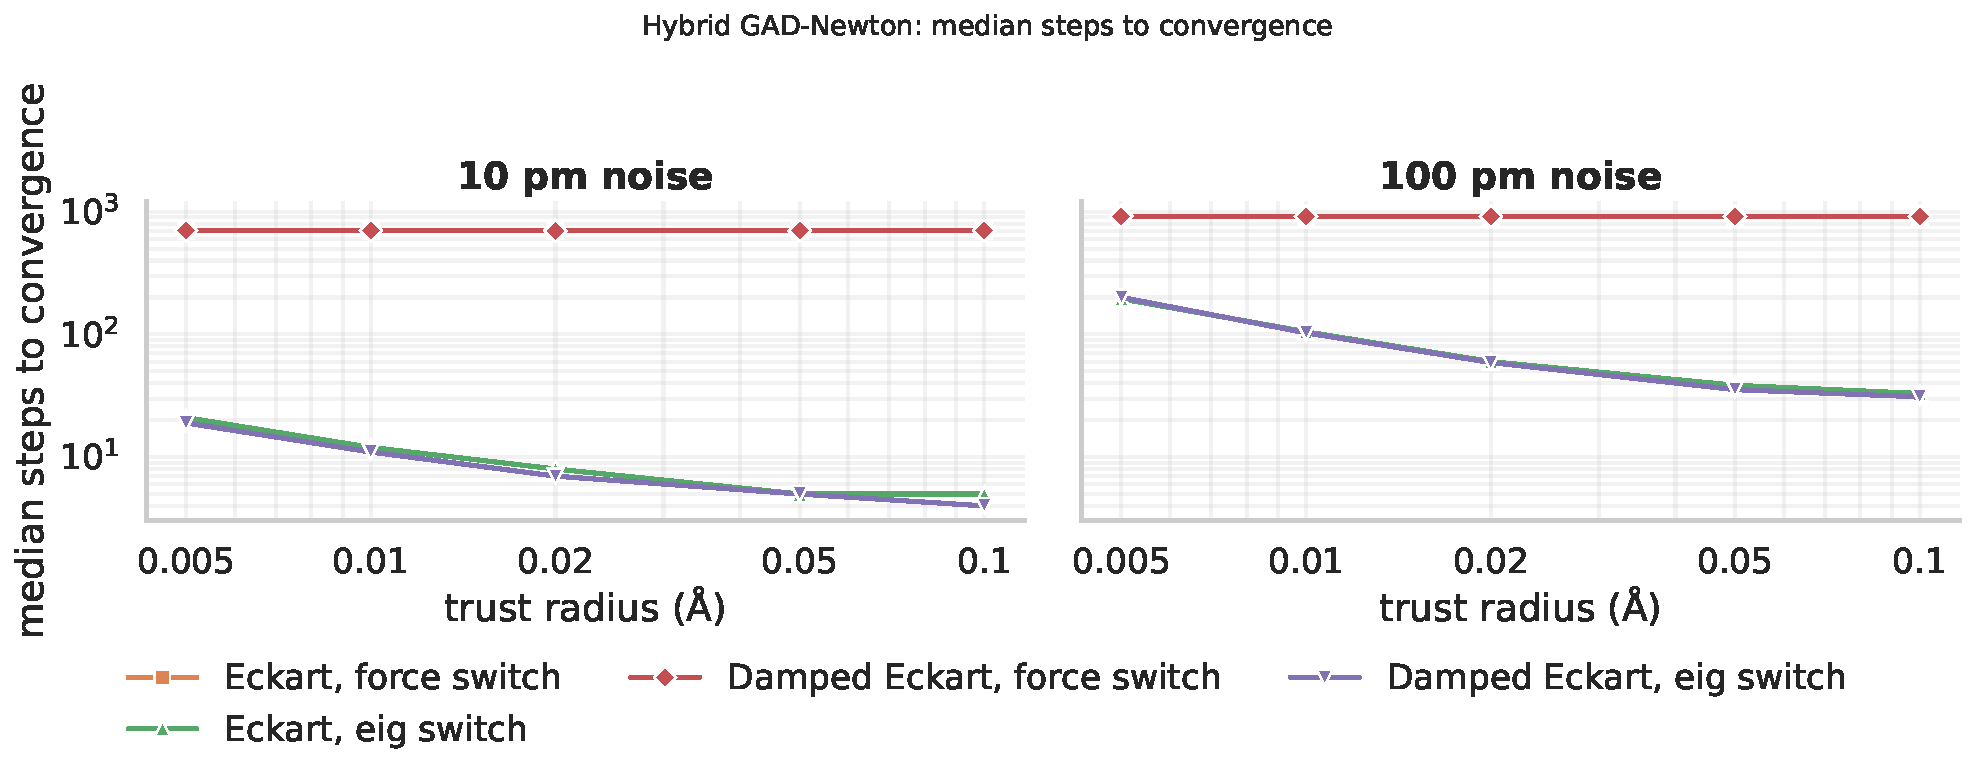
\includegraphics[width=\textwidth]{figures/fig_hybrid_steps_vs_tr.pdf}
\caption{Median steps to converge as a function of trust radius. Y-axis
log-scaled. The switch=True curves drop \emph{monotonically} with
trust radius (4 vs 21 at 10pm; 31 vs 200 at 100pm) --- larger tr lets
Newton take bigger first steps. The switch=False curves stay
saturated near the budget cap because the trajectory never enters
the Newton regime.}
\end{figure}

\begin{figure}[H]
\centering
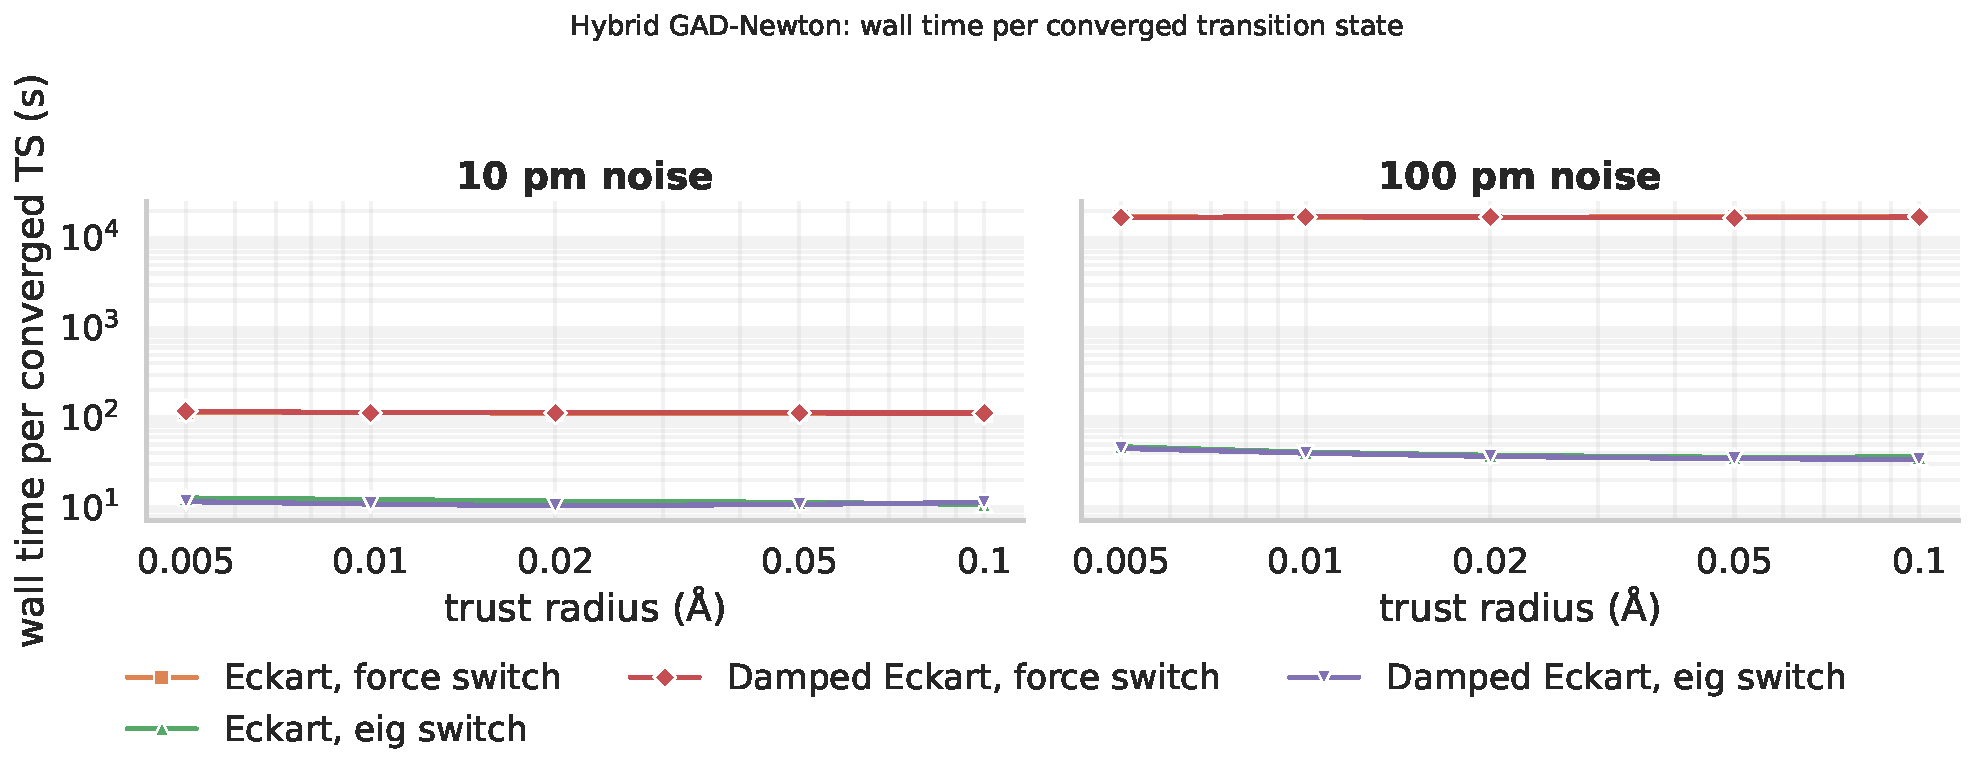
\includegraphics[width=\textwidth]{figures/fig_hybrid_wall_vs_tr.pdf}
\caption{Wall-time per converged TS. The switch=False rows are
two orders of magnitude slower than switch=True at 100pm (because
the denominator $n_{\text{conv}}$ is 1 vs $\sim$190); at 10pm the gap
is 10$\times$. switch=True saturates at $\sim$10s/conv at 10pm and
$\sim$35s/conv at 100pm.}
\end{figure}

% =================================================================
\section*{Sources for every number}
% =================================================================

See \texttt{analysis\_2026\_04\_29/hybrid\_gad\_newton\_pivot.md} for the
machine-readable pivots.

\begin{itemize}[leftmargin=1.5em, itemsep=0.05em]
\item Per-cell summary parquets:
  \texttt{runs/hybrid\_gad\_newton\_rerun\_fixed/<method\_tag>\_<noise>pm/summary\_*.parquet}
\item Aggregator:
  \texttt{analysis\_2026\_04\_29/hybrid\_gad\_newton\_summary.csv}
  (40 rows, one per cell).
\item Build script: \texttt{scripts/analyze\_hybrid\_gad\_newton.py}.
\item Standalone runner: \texttt{scripts/hybrid\_gad\_newton\_runner.py}.
\item SLURM array: \texttt{scripts/run\_hybrid\_gad\_newton.slurm}
  (job 60460000, tasks 10--49).
\item Step-function source files: see "What this sweep does" above.
\item Bug fix: commit \texttt{a80a763}, "return cartesian coord steps in hybrid".
\item \textbf{Sella baselines} (used in the side-by-side table):
  \texttt{analysis\_2026\_04\_29/test\_summary\_full.csv}, filtered to
  \texttt{noise\_pm}$\in$\{10, 100\} and aggregated with
  conv = \texttt{is\_saddle} $\wedge$ \texttt{fmax\_loose}
  ($\equiv n_{\text{neg}}{=}1 \wedge f_{\max}{<}0.01$).
  Source runs: \texttt{runs/sella\_2000/} (cart+Eckart \emph{libdef},
  cart no-Eckart \emph{default}, internal-coord \emph{internal}).
\item \textbf{Plain GAD baselines}: from the main report's
  \texttt{gad\_dt00\{3,5,7\}\_fmax} runs at the 5000-step budget;
  numbers reproduced in
  \texttt{analysis\_2026\_04\_29/hybrid\_gad\_newton\_pivot.md}.
\end{itemize}

\end{document}
